\documentclass[crop=false,class=article,oneside]{standalone}
%----------------------------Preamble-------------------------------%
%---------------------------Packages----------------------------%
\usepackage{geometry}
\geometry{b5paper, margin=1.0in}
\usepackage[T1]{fontenc}
\usepackage{graphicx, float}            % Graphics/Images.
\usepackage{natbib}                     % For bibliographies.
\bibliographystyle{agsm}                % Bibliography style.
\usepackage[french, english]{babel}     % Language typesetting.
\usepackage[dvipsnames]{xcolor}         % Color names.
\usepackage{listings}                   % Verbatim-Like Tools.
\usepackage{mathtools, esint, mathrsfs} % amsmath and integrals.
\usepackage{amsthm, amsfonts, amssymb}  % Fonts and theorems.
\usepackage{tcolorbox}                  % Frames around theorems.
\usepackage{upgreek}                    % Non-Italic Greek.
\usepackage{fmtcount, etoolbox}         % For the \book{} command.
\usepackage[newparttoc]{titlesec}       % Formatting chapter, etc.
\usepackage{titletoc}                   % Allows \book in toc.
\usepackage[nottoc]{tocbibind}          % Bibliography in toc.
\usepackage[titles]{tocloft}            % ToC formatting.
\usepackage{pgfplots, tikz}             % Drawing/graphing tools.
\usepackage{imakeidx}                   % Used for index.
\usetikzlibrary{
    calc,                   % Calculating right angles and more.
    angles,                 % Drawing angles within triangles.
    arrows.meta,            % Latex and Stealth arrows.
    quotes,                 % Adding labels to angles.
    positioning,            % Relative positioning of nodes.
    decorations.markings,   % Adding arrows in the middle of a line.
    patterns,
    arrows
}                                       % Libraries for tikz.
\pgfplotsset{compat=1.9}                % Version of pgfplots.
\usepackage[font=scriptsize,
            labelformat=simple,
            labelsep=colon]{subcaption} % Subfigure captions.
\usepackage[font={scriptsize},
            hypcap=true,
            labelsep=colon]{caption}    % Figure captions.
\usepackage[pdftex,
            pdfauthor={Ryan Maguire},
            pdftitle={Mathematics and Physics},
            pdfsubject={Mathematics, Physics, Science},
            pdfkeywords={Mathematics, Physics, Computer Science, Biology},
            pdfproducer={LaTeX},
            pdfcreator={pdflatex}]{hyperref}
\hypersetup{
    colorlinks=true,
    linkcolor=blue,
    filecolor=magenta,
    urlcolor=Cerulean,
    citecolor=SkyBlue
}                           % Colors for hyperref.
\usepackage[toc,acronym,nogroupskip,nopostdot]{glossaries}
\usepackage{glossary-mcols}
%------------------------Theorem Styles-------------------------%
\theoremstyle{plain}
\newtheorem{theorem}{Theorem}[section]

% Define theorem style for default spacing and normal font.
\newtheoremstyle{normal}
    {\topsep}               % Amount of space above the theorem.
    {\topsep}               % Amount of space below the theorem.
    {}                      % Font used for body of theorem.
    {}                      % Measure of space to indent.
    {\bfseries}             % Font of the header of the theorem.
    {}                      % Punctuation between head and body.
    {.5em}                  % Space after theorem head.
    {}

% Italic header environment.
\newtheoremstyle{thmit}{\topsep}{\topsep}{}{}{\itshape}{}{0.5em}{}

% Define environments with italic headers.
\theoremstyle{thmit}
\newtheorem*{solution}{Solution}

% Define default environments.
\theoremstyle{normal}
\newtheorem{example}{Example}[section]
\newtheorem{definition}{Definition}[section]
\newtheorem{problem}{Problem}[section]

% Define framed environment.
\tcbuselibrary{most}
\newtcbtheorem[use counter*=theorem]{ftheorem}{Theorem}{%
    before=\par\vspace{2ex},
    boxsep=0.5\topsep,
    after=\par\vspace{2ex},
    colback=green!5,
    colframe=green!35!black,
    fonttitle=\bfseries\upshape%
}{thm}

\newtcbtheorem[auto counter, number within=section]{faxiom}{Axiom}{%
    before=\par\vspace{2ex},
    boxsep=0.5\topsep,
    after=\par\vspace{2ex},
    colback=Apricot!5,
    colframe=Apricot!35!black,
    fonttitle=\bfseries\upshape%
}{ax}

\newtcbtheorem[use counter*=definition]{fdefinition}{Definition}{%
    before=\par\vspace{2ex},
    boxsep=0.5\topsep,
    after=\par\vspace{2ex},
    colback=blue!5!white,
    colframe=blue!75!black,
    fonttitle=\bfseries\upshape%
}{def}

\newtcbtheorem[use counter*=example]{fexample}{Example}{%
    before=\par\vspace{2ex},
    boxsep=0.5\topsep,
    after=\par\vspace{2ex},
    colback=red!5!white,
    colframe=red!75!black,
    fonttitle=\bfseries\upshape%
}{ex}

\newtcbtheorem[auto counter, number within=section]{fnotation}{Notation}{%
    before=\par\vspace{2ex},
    boxsep=0.5\topsep,
    after=\par\vspace{2ex},
    colback=SeaGreen!5!white,
    colframe=SeaGreen!75!black,
    fonttitle=\bfseries\upshape%
}{not}

\newtcbtheorem[use counter*=remark]{fremark}{Remark}{%
    fonttitle=\bfseries\upshape,
    colback=Goldenrod!5!white,
    colframe=Goldenrod!75!black}{ex}

\newenvironment{bproof}{\textit{Proof.}}{\hfill$\square$}
\tcolorboxenvironment{bproof}{%
    blanker,
    breakable,
    left=3mm,
    before skip=5pt,
    after skip=10pt,
    borderline west={0.6mm}{0pt}{green!80!black}
}

\AtEndEnvironment{lexample}{$\hfill\textcolor{red}{\blacksquare}$}
\newtcbtheorem[use counter*=example]{lexample}{Example}{%
    empty,
    title={Example~\theexample},
    boxed title style={%
        empty,
        size=minimal,
        toprule=2pt,
        top=0.5\topsep,
    },
    coltitle=red,
    fonttitle=\bfseries,
    parbox=false,
    boxsep=0pt,
    before=\par\vspace{2ex},
    left=0pt,
    right=0pt,
    top=3ex,
    bottom=1ex,
    before=\par\vspace{2ex},
    after=\par\vspace{2ex},
    breakable,
    pad at break*=0mm,
    vfill before first,
    overlay unbroken={%
        \draw[red, line width=2pt]
            ([yshift=-1.2ex]title.south-|frame.west) to
            ([yshift=-1.2ex]title.south-|frame.east);
        },
    overlay first={%
        \draw[red, line width=2pt]
            ([yshift=-1.2ex]title.south-|frame.west) to
            ([yshift=-1.2ex]title.south-|frame.east);
    },
}{ex}

\AtEndEnvironment{ldefinition}{$\hfill\textcolor{Blue}{\blacksquare}$}
\newtcbtheorem[use counter*=definition]{ldefinition}{Definition}{%
    empty,
    title={Definition~\thedefinition:~{#1}},
    boxed title style={%
        empty,
        size=minimal,
        toprule=2pt,
        top=0.5\topsep,
    },
    coltitle=Blue,
    fonttitle=\bfseries,
    parbox=false,
    boxsep=0pt,
    before=\par\vspace{2ex},
    left=0pt,
    right=0pt,
    top=3ex,
    bottom=0pt,
    before=\par\vspace{2ex},
    after=\par\vspace{1ex},
    breakable,
    pad at break*=0mm,
    vfill before first,
    overlay unbroken={%
        \draw[Blue, line width=2pt]
            ([yshift=-1.2ex]title.south-|frame.west) to
            ([yshift=-1.2ex]title.south-|frame.east);
        },
    overlay first={%
        \draw[Blue, line width=2pt]
            ([yshift=-1.2ex]title.south-|frame.west) to
            ([yshift=-1.2ex]title.south-|frame.east);
    },
}{def}

\AtEndEnvironment{ltheorem}{$\hfill\textcolor{Green}{\blacksquare}$}
\newtcbtheorem[use counter*=theorem]{ltheorem}{Theorem}{%
    empty,
    title={Theorem~\thetheorem:~{#1}},
    boxed title style={%
        empty,
        size=minimal,
        toprule=2pt,
        top=0.5\topsep,
    },
    coltitle=Green,
    fonttitle=\bfseries,
    parbox=false,
    boxsep=0pt,
    before=\par\vspace{2ex},
    left=0pt,
    right=0pt,
    top=3ex,
    bottom=-1.5ex,
    breakable,
    pad at break*=0mm,
    vfill before first,
    overlay unbroken={%
        \draw[Green, line width=2pt]
            ([yshift=-1.2ex]title.south-|frame.west) to
            ([yshift=-1.2ex]title.south-|frame.east);},
    overlay first={%
        \draw[Green, line width=2pt]
            ([yshift=-1.2ex]title.south-|frame.west) to
            ([yshift=-1.2ex]title.south-|frame.east);
    }
}{thm}

%--------------------Declared Math Operators--------------------%
\DeclareMathOperator{\adjoint}{adj}         % Adjoint.
\DeclareMathOperator{\Card}{Card}           % Cardinality.
\DeclareMathOperator{\curl}{curl}           % Curl.
\DeclareMathOperator{\diam}{diam}           % Diameter.
\DeclareMathOperator{\dist}{dist}           % Distance.
\DeclareMathOperator{\Div}{div}             % Divergence.
\DeclareMathOperator{\Erf}{Erf}             % Error Function.
\DeclareMathOperator{\Erfc}{Erfc}           % Complementary Error Function.
\DeclareMathOperator{\Ext}{Ext}             % Exterior.
\DeclareMathOperator{\GCD}{GCD}             % Greatest common denominator.
\DeclareMathOperator{\grad}{grad}           % Gradient
\DeclareMathOperator{\Ima}{Im}              % Image.
\DeclareMathOperator{\Int}{Int}             % Interior.
\DeclareMathOperator{\LC}{LC}               % Leading coefficient.
\DeclareMathOperator{\LCM}{LCM}             % Least common multiple.
\DeclareMathOperator{\LM}{LM}               % Leading monomial.
\DeclareMathOperator{\LT}{LT}               % Leading term.
\DeclareMathOperator{\Mod}{mod}             % Modulus.
\DeclareMathOperator{\Mon}{Mon}             % Monomial.
\DeclareMathOperator{\multideg}{mutlideg}   % Multi-Degree (Graphs).
\DeclareMathOperator{\nul}{nul}             % Null space of operator.
\DeclareMathOperator{\Ord}{Ord}             % Ordinal of ordered set.
\DeclareMathOperator{\Prin}{Prin}           % Principal value.
\DeclareMathOperator{\proj}{proj}           % Projection.
\DeclareMathOperator{\Refl}{Refl}           % Reflection operator.
\DeclareMathOperator{\rk}{rk}               % Rank of operator.
\DeclareMathOperator{\sgn}{sgn}             % Sign of a number.
\DeclareMathOperator{\sinc}{sinc}           % Sinc function.
\DeclareMathOperator{\Span}{Span}           % Span of a set.
\DeclareMathOperator{\Spec}{Spec}           % Spectrum.
\DeclareMathOperator{\supp}{supp}           % Support
\DeclareMathOperator{\Tr}{Tr}               % Trace of matrix.
%--------------------Declared Math Symbols--------------------%
\DeclareMathSymbol{\minus}{\mathbin}{AMSa}{"39} % Unary minus sign.
%------------------------New Commands---------------------------%
\DeclarePairedDelimiter\norm{\lVert}{\rVert}
\DeclarePairedDelimiter\ceil{\lceil}{\rceil}
\DeclarePairedDelimiter\floor{\lfloor}{\rfloor}
\newcommand*\diff{\mathop{}\!\mathrm{d}}
\newcommand*\Diff[1]{\mathop{}\!\mathrm{d^#1}}
\renewcommand*{\glstextformat}[1]{\textcolor{RoyalBlue}{#1}}
\renewcommand{\glsnamefont}[1]{\textbf{#1}}
\renewcommand\labelitemii{$\circ$}
\renewcommand\thesubfigure{%
    \arabic{chapter}.\arabic{figure}.\arabic{subfigure}}
\addto\captionsenglish{\renewcommand{\figurename}{Fig.}}
\numberwithin{equation}{section}

\renewcommand{\vector}[1]{\boldsymbol{\mathrm{#1}}}

\newcommand{\uvector}[1]{\boldsymbol{\hat{\mathrm{#1}}}}
\newcommand{\topspace}[2][]{(#2,\tau_{#1})}
\newcommand{\measurespace}[2][]{(#2,\varSigma_{#1},\mu_{#1})}
\newcommand{\measurablespace}[2][]{(#2,\varSigma_{#1})}
\newcommand{\manifold}[2][]{(#2,\tau_{#1},\mathcal{A}_{#1})}
\newcommand{\tanspace}[2]{T_{#1}{#2}}
\newcommand{\cotanspace}[2]{T_{#1}^{*}{#2}}
\newcommand{\Ckspace}[3][\mathbb{R}]{C^{#2}(#3,#1)}
\newcommand{\funcspace}[2][\mathbb{R}]{\mathcal{F}(#2,#1)}
\newcommand{\smoothvecf}[1]{\mathfrak{X}(#1)}
\newcommand{\smoothonef}[1]{\mathfrak{X}^{*}(#1)}
\newcommand{\bracket}[2]{[#1,#2]}

%------------------------Book Command---------------------------%
\makeatletter
\renewcommand\@pnumwidth{1cm}
\newcounter{book}
\renewcommand\thebook{\@Roman\c@book}
\newcommand\book{%
    \if@openright
        \cleardoublepage
    \else
        \clearpage
    \fi
    \thispagestyle{plain}%
    \if@twocolumn
        \onecolumn
        \@tempswatrue
    \else
        \@tempswafalse
    \fi
    \null\vfil
    \secdef\@book\@sbook
}
\def\@book[#1]#2{%
    \refstepcounter{book}
    \addcontentsline{toc}{book}{\bookname\ \thebook:\hspace{1em}#1}
    \markboth{}{}
    {\centering
     \interlinepenalty\@M
     \normalfont
     \huge\bfseries\bookname\nobreakspace\thebook
     \par
     \vskip 20\p@
     \Huge\bfseries#2\par}%
    \@endbook}
\def\@sbook#1{%
    {\centering
     \interlinepenalty \@M
     \normalfont
     \Huge\bfseries#1\par}%
    \@endbook}
\def\@endbook{
    \vfil\newpage
        \if@twoside
            \if@openright
                \null
                \thispagestyle{empty}%
                \newpage
            \fi
        \fi
        \if@tempswa
            \twocolumn
        \fi
}
\newcommand*\l@book[2]{%
    \ifnum\c@tocdepth >-3\relax
        \addpenalty{-\@highpenalty}%
        \addvspace{2.25em\@plus\p@}%
        \setlength\@tempdima{3em}%
        \begingroup
            \parindent\z@\rightskip\@pnumwidth
            \parfillskip -\@pnumwidth
            {
                \leavevmode
                \Large\bfseries#1\hfill\hb@xt@\@pnumwidth{\hss#2}
            }
            \par
            \nobreak
            \global\@nobreaktrue
            \everypar{\global\@nobreakfalse\everypar{}}%
        \endgroup
    \fi}
\newcommand\bookname{Book}
\renewcommand{\thebook}{\texorpdfstring{\Numberstring{book}}{book}}
\providecommand*{\toclevel@book}{-2}
\makeatother
\titleformat{\part}[display]
    {\Large\bfseries}
    {\partname\nobreakspace\thepart}
    {0mm}
    {\Huge\bfseries}
\titlecontents{part}[0pt]
    {\large\bfseries}
    {\partname\ \thecontentslabel: \quad}
    {}
    {\hfill\contentspage}
\titlecontents{chapter}[0pt]
    {\bfseries}
    {\chaptername\ \thecontentslabel:\quad}
    {}
    {\hfill\contentspage}
\newglossarystyle{longpara}{%
    \setglossarystyle{long}%
    \renewenvironment{theglossary}{%
        \begin{longtable}[l]{{p{0.25\hsize}p{0.65\hsize}}}
    }{\end{longtable}}%
    \renewcommand{\glossentry}[2]{%
        \glstarget{##1}{\glossentryname{##1}}%
        &\glossentrydesc{##1}{~##2.}
        \tabularnewline%
        \tabularnewline
    }%
}
\newglossary[not-glg]{notation}{not-gls}{not-glo}{Notation}
\newcommand*{\newnotation}[4][]{%
    \newglossaryentry{#2}{type=notation, name={\textbf{#3}, },
                          text={#4}, description={#4},#1}%
}
%--------------------------LENGTHS------------------------------%
% Spacings for the Table of Contents.
\addtolength{\cftsecnumwidth}{1ex}
\addtolength{\cftsubsecindent}{1ex}
\addtolength{\cftsubsecnumwidth}{1ex}
\addtolength{\cftfignumwidth}{1ex}
\addtolength{\cfttabnumwidth}{1ex}

% Indent and paragraph spacing.
\setlength{\parindent}{0em}
\setlength{\parskip}{0em}
%--------------------------Main Document----------------------------%
\begin{document}
    \ifx\ifsub\undefined
        \section*{Convexity: Part I}
        \setcounter{section}{1}
    \fi
    \subsection{Convexity in the Euclidean Plane}
        \begin{definition}
        $A(K)$ is the area of a compact set $K$.
        \end{definition}
        \begin{definition}
        The perimeter $P(K)$ is the length of the boundary curve, $\mu(\partial K)$.
        \end{definition}
        \begin{definition}
        The section $X_{\ell}(K)$ is defined for any given straight line $\ell$ to be the length $\mu(K\cap \ell)$.
        \end{definition}
        \begin{definition}
        Given a straight line $\ell$, the width $W_{\ell}(K)$ is $\mu(\ell_{K})$.
        \end{definition}
        \begin{definition}
        The mean width $W(K)$ is the average of the width of all $W_{\ell}(K)$.
        \end{definition}
        \begin{definition}
        The minimum width $w(K)$ is the minimum of $W_{\ell}(K)$ over all possible directions of the line $\ell$.
        \end{definition}
        \begin{definition}
        The maximum width $\check{W}$ is the maximum of $W_{\ell}(K)$.
        \end{definition}
        \begin{definition}
        The diameter $D(K)$ is the maximum distance between any two points inside $K$.
        \end{definition}
        \begin{definition}
        The inradius $r_K$ is the maximum radius of any circle inside $K$.
        \end{definition}
        \begin{definition}
        The circumradius $R_K$ is the minimum radius of any circle containing $K$.
        \end{definition}
        \begin{notation}
        For bounded sets $K\subset \mathbb{R}^2$, define $R_K(\theta)$ as the projection or $K$ onto the line $\sin(\theta)y=\cos(\theta)x$.
        \end{notation}
        \begin{theorem}
        If $K$ is a compact subset of $\mathbb{R}^n$, then there are points $x,y\in K$ such that $d(x,y)=D(K)$.
        \end{theorem}
        \begin{proof}
        As $K$ is compact, it is bounded. Let $M$ be such a bound. Then the set $D=\{r\in \mathbb{R}^+| d(x,y) = r,\ x,y\in K\}$ is bounded by $M$. Let $d$ be the least upper bound of this set. Then we can find a sequence of points $x_n,y_n\in K$ such that $d(x_n,y_n) \rightarrow d$. As $K$ is compact, there are convergent subsequence $x_{n_k}$ and $y_{n_k}$ with limits in $K$, call them $x$ and $y$. Then $d(x,y) = d$. Thus, there are points $x,y\in K$ such that $d(x,y) \geq d(a,b)$ for all $a,b\in K$. Therefore $D(K)$ is equal to $d$.
        \end{proof}
        \begin{theorem}
        There exist bounded sets $K$ such that $R_K(\theta)$ is not continuous.
        \end{theorem}
        \begin{proof}
        For define $\mathcal{M} = \{(x,y)\in [-1,1]^2: x\in \mathbb{Q},y\in \mathbb{R}\}$, and let $\mathcal{N} = \{(x,y)\in \mathbb{R}^2: x^2+y^2\leq 1\}$, and consider $K = \mathcal{M}\cap \mathcal{N}$. $f_{K}(\theta)$ is discontinuous at $\theta = \frac{\pi}{2}$. For, $f_K(\frac{\pi}{2}) = \mu(\mathbb{Q}\cap [-1,1])=0$. But, for any $0<\delta < \pi$, $f_K(\frac{\pi}{2}\pm\delta) = 2$. Thus, $f_K(\theta) = \begin{cases} 0, & \theta = \pm \frac{\pi}{2} \\ 2, & \theta \ne \pm \frac{\pi}{2}\end{cases}$. In the image below, the length of $R_K(\frac{\pi}{2}-\delta)$ is the length of the line $\overline{AB}$, which is 2.
        \end{proof}
        \begin{figure}[H]
          \begin{subfigure}[b]{0.32\textwidth}
             \centering
            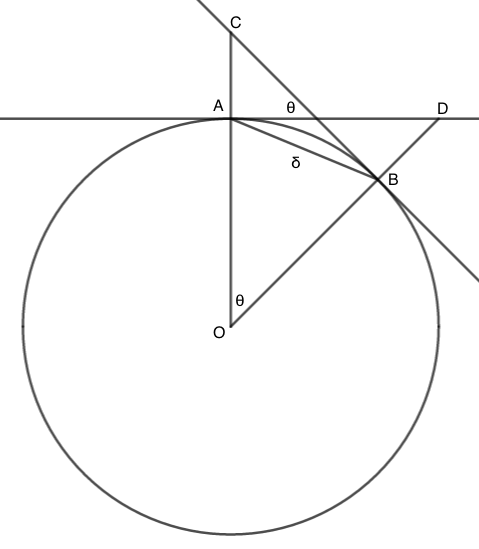
\includegraphics[width=\textwidth]{Circle-1.png}
            \caption{Drawing for Theorem 3.2.2}
          \end{subfigure}
          \begin{subfigure}[b]{0.32\textwidth}
            \centering
            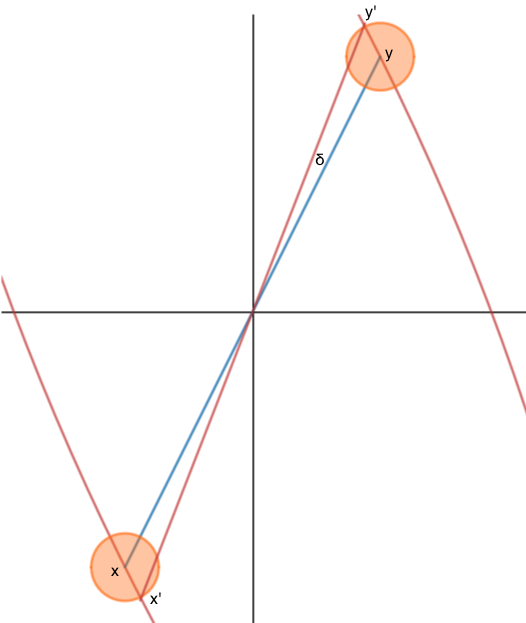
\includegraphics[width=\textwidth]{convex-1.png}
            \caption{Drawing for Theorem 3.2.3}
          \end{subfigure}
          \begin{subfigure}[b]{0.32\textwidth}
            \centering
            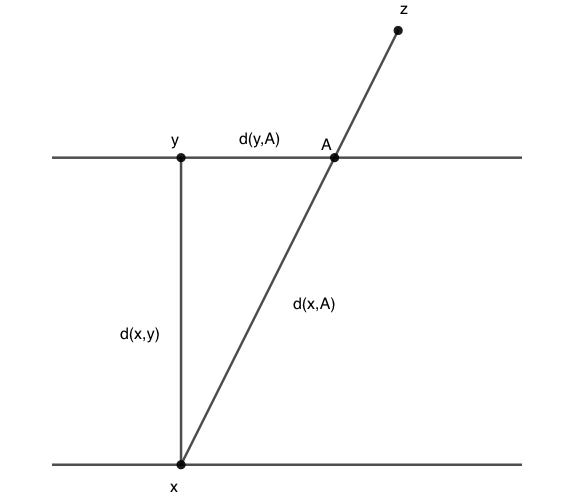
\includegraphics[width=\textwidth]{line-1.png}
            \caption{Drawing for Lemma 3.2.1}
          \end{subfigure}  
        \end{figure}
        \begin{theorem}
        If $K\subset \mathbb{R}^2$ is compact and convex, then $R_K(\theta)$ is continuous.
        \end{theorem}
        \begin{proof}
        For let $K$ be compact and convex, and without loss of generality suppose it contained within the unit disc and contains the origin. Let $\theta\in (0,2\pi)$ be given and let $\ell_{\theta}$ be a line through the origin making an angle $\theta$ with the horizontal. Let $x=(x_1,x_2),y=(y_1,y_2)\in K$ be such that $W_{\ell_{\theta}}(K) = d(x,y)$. Such points exist as $K$ is compact. Let $\varepsilon>0$ be given. About $x$, consider $B_{\frac{\varepsilon}{2}}(x)$, and similarly $B_{\frac{\varepsilon}{2}}(y)$. Neither of these are empty, as $K$ is convex. Let $x',y'\in K\cap(B_{\frac{\varepsilon}{2}}(x)\cup B_{\frac{\varepsilon}{2}}(y))$ be such that $d(x',y')$ is maximized. As this set is compact, such points exist. Let $\delta = \min\{|\theta-\frac{x_2'}{\sqrt{x_1'^2+x_2'^2}}|,|\theta-\frac{y_2'}{\sqrt{y_1'^2+y_2'^2}}|\}$. Then for $|\theta-\theta_0|<\delta$, $d(x,y)-\varepsilon \leq W_{\ell_{\theta_0}}(K)\leq d(x,y)+\varepsilon$, and thus $|W_{\ell_\theta}(K)-W_{\ell_{\theta_0}}(K)| < \varepsilon$.
        \end{proof}
        \begin{lemma}
        If $K$ is a compact subset of $\mathbb{R}^2$ and $x,y\in K$ such that $d(x,y)=D(K)$, then the lines perpendicular to $\overline{xy}$ at $x$ and $y$ contain all of $K$ in between.
        \end{lemma}
        \begin{proof}
        Suppose not. Let $\overline{X}$ be the line perpendicular to $\overline{xy}$ containing point $x$, and similarly define $\overline{Y}$. Suppose there is a point $z\in K$ that falls on the exterior of the region $\mathcal{U} = \{(x,y)\in \mathbb{R}^2: (x,y)\ \textrm{Lies Between } \overline{X}\ \textrm{and } \overline{Y}\}$. Note that $d(x,z)\ne d(y,z)$, as then $z$ would line between these two lines. Suppose $d(y,z)<d(x,z)$. Where the line $\overline{xz}$ cuts $\overline{Y}$ denote as $A$. But then $d(x,z) > d(x,A) = \sqrt{d(y,A)^2+d(x,y)^2}\geq d(x,y)$. A contradiction as $d(x,y) = D(K)$. Thus $z\in \mathcal{U}$.
        \end{proof}
        \begin{theorem}
        If $K\subset \mathbb{R}^2$ is compact and convex, then there are points $x,y\in K$ such that $\check{W}(K)=d(x,y)$.
        \end{theorem}
        \begin{proof}
        As $f_K(\theta)$ is continuous for convex compact set, and as it is continuous on a compact set $[0,2\pi]$, it attains its maximum. Let $\theta$ be such a maximum. Let $\ell_{\theta}$ be the line through the origin which makes an angle $\theta$ with the horizontal axis and consider set $K_{\ell_{\theta}}$. As $K$ is compact and $\ell_{\theta}$ is closed, $K_{\ell_{\theta}}$ is compact. Then $W=\{d(x,y):x,y\in K_{\ell_{\theta}}\}$ is bounded, has a least upper bound, and therefore there are points $x,y \in K$ such that $\check{W}(K)=d(x,y)$.
        \end{proof}
        \begin{theorem}
        If $K$ is a compact convex set of $\mathbb{R}^2$, then $D(K) = \check{W}(K)$.
        \end{theorem}
        \begin{proof}
        As $K$ is compact, $D(K)$ and $\check{W}(K)$ exists and there are points $x,y$ such that $d(x,y) = D(K)$ and points $x',y'$ such that $d(x',y') = \check{W}(K)$. Suppose $d(x',y')> d(x,y)$. A contradiction, as $d(x,y)$ is the diameter of $K$. So $d(x,y) \geq d(x',y')$. Now suppose $d(x,y)>d(x',y')$. But as $d(x',y')= \check{W}(K)$, $d(x',y')$ is the greatest length of any line segment that terminates in $K$ and such that perpendiculars at these terminating points contain all of $K$. But as $d(x,y)=D(K)$, the lines perpendicular to $\overline{xy}$ at $x$ and $y$ contain all of $K$, a contradiction. Thus $d(x',y') \geq d(x,y)$. But it was just showed that $d(x,y)\geq d(x',y')$. Thus, $d(x,y) = d(x',y')$. $D(K) = \check{W}(K)$.
        \end{proof}
        \begin{definition}
        If $Q$ is a convex polygon with interior (That is, positive area) in $\mathbb{R}^2$, then the perimeter of $Q$ is the sum of the lengths of its edges. 
        \end{definition}
        \begin{definition}
        The perimeter of a line segment $e$ is $P(e) = 2|e|$.
        \end{definition}
        \begin{remark}
        This is for the sake of continuity. If we take a rectangle of length $|e|$ and width $\frac{1}{n}$, then the perimeter is $2|e|+\frac{2}{n} \rightarrow 2|e|$ as $n\rightarrow \infty$. Thus, for the puprose of continuity we define the perimeter of line segments to be twice their length.
        \end{remark}
        \begin{theorem}[Cauchy's Perimeter Theorem]
        If $K$ is a compact convex subset of the plane, then $P(K) = \pi W(K)$.
        \end{theorem}
        \begin{proof}
        Suppose that $Q$ is a convex polygon with edges $e_1,\hdots, e_n$. At each $e_i$, let $\theta_i$ be the angle made with $e_i$ and the horizontal axis of $\mathbb{R}^2$. The mean width is $W(Q) = \frac{1}{2\pi}\int_{0}^{2\pi} W_{\ell_\theta}(Q)d\theta = \frac{1}{2\pi} \int_{0}^{2\pi} \frac{1}{2} \sum_{i=1}^{n} |e_i||\cos(\theta-\theta_i)|d\theta = \frac{1}{4\pi}\sum_{i=1}^{n} |e_i|\int_{0}^{2\pi} |\cos(\theta-\theta_i)|d\theta = \frac{1}{\pi} \sum_{i=1}^{n} |e_i| = \frac{1}{\pi} P(Q)$. Thus, $P(Q) = \pi W(Q)$. For any convex compact subset $K\subset \mathbb{R}^2$, we may find a polygon $Q$ that approximates the boundary with a perimeter $P(Q)$ that is as close to $P(K)$ and a width $W(Q)$ as close to $W(K)$ as desired. That is, for all $n\in \mathbb{N}$, we can obtain a polynomial $Q_n$ such that $\max\{|W(Q_n)-W(K)|,|P(K)-P(Q_n)|\}< \frac{1}{n}$. Then $|P(K)-\pi W(K)| = |P(K) - P(Q_n)+P(Q_n)-\pi W(Q_n)+\pi W(Q_n)-\pi W(K)| \leq |P(K)-P(Q_n)|+|P(Q_n)-\pi W(Q_n)|+\pi|W(Q_n)-W(K)| < \frac{1}{n} + 0 + \frac{\pi}{n} = \frac{1+\pi}{n} \rightarrow 0$. Thus, $P(K) = \pi W(K)$ for arbitrary convex compact subsets of the plane.
        \end{proof}
        \begin{theorem}
        There exist compact path-connected sets $K\subset \mathbb{R}^2$ such that $P(K) \ne \pi W(K)$.
        \end{theorem}
        \begin{proof}
        Consider the set $K = \{(x,y) \in \mathbb{R}^2: x^2+y^2=1, y\geq 0\}$. Then $P(K) = 2\pi$, but \\ $W(K) = \pi(\pi+2)$. To see this, consider the set $\mathcal{K} = \{(x,y)\in \mathbb{R}^2: x^2 + y^2 \leq 1, y\geq 0\}$. This is convex and has perimeter $\pi+2$ and therefore $W(\mathcal{K}) = \pi(\pi+2)$. But, as the image shows, $W(K) = W(\mathcal{K})$. That is, $W_{\ell_{\theta}}(K)$ is the length of the line segment $\overline{AB}$, as is $W_{\ell_{\theta}}(\mathcal{K})$. Therefore the averages $W(K)$ and $W(\mathcal{K})$ are the same. Thus, $P(K) \ne \pi W(K)$.
        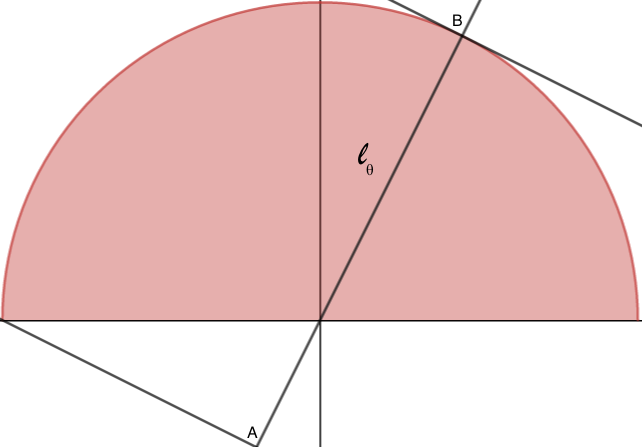
\includegraphics[scale=0.3]{semicircle-1.png}
        \end{proof}
        \begin{definition}
        A functional $f$ with respect to subset inclusion is said to be monotonic on a family of sets $\mathscr{P}$ if and only if $f(K)\leq f(L)$ for all $K,L \in \mathscr{P}$ such that $K\subset L$.
        \end{definition}
        \begin{theorem}
        If $K\subset L \in \mathscr{K}_2$, then $W_{\ell}(K) \leq W_{\ell}(L)$.
        \end{theorem}
        \begin{proof}
        For let $\pi_{\ell}:\mathbb{R}^2 \rightarrow \ell$ be the orthogonal projection map of $\mathbb{R}^2$ to $\ell$. Then $\pi_{\ell}(K)\leq \pi_{\ell}(L)$ as $K\subset L$, and thus $W_{\ell}(K)\leq W_{\ell}(L)$.
        \end{proof}
        \begin{theorem}
        If $K\subset L\in \mathscr{K}_2$, then $W(K)\leq W(L)$.
        \end{theorem}
        \begin{proof}
        For $W_{\ell}(K)\leq W_{\ell}(L)$, and thus $W(K)=\frac{1}{2\pi}\int_{0}^{2\pi}W_{\ell_{\theta}}(K)d\theta \leq \frac{1}{2\pi}\int_{0}^{2\pi}W_{\ell_{\theta}}(L)d\theta=W(L)$.
        \end{proof}
        \begin{theorem}
        If $K\subset L\in \mathscr{K}_2$, then $X_{\ell}(K)\leq X_{\ell}(L)$.
        \end{theorem}
        \begin{proof}
        For if $x\in \ell\cap K$, then $x\in \ell\cap L$, and thus $X_{\ell}(K)=\mu(\ell\cap K) \leq \mu(\ell\cap L)=X_{\ell}(L)$.
        \end{proof}
        \begin{theorem}
        If $K\subset L\subset \mathscr{K}_2$, then $D(K)\leq D(L)$.
        \end{theorem}
        \begin{proof}
        For suppose not. Suppose $D(K)>D(L)$. Then, there are points $x,y\in K$ such that $d(x,y)> \sup\{d(x',y'):x',y'\in L\}$. But as $K\subset L$, $x,y\in L$ and thus $d(x,y) \not> \sup\{d(x',y'):x',y'\in L\}$. Thus, $D(K)\leq D(L)$.
        \end{proof}
        \begin{theorem}
        If $K\subset L \subset \mathscr{K}_2$, then $R_K\leq R_L$.
        \end{theorem}
        \begin{proof}
        For suppose not. Suppose $R_K>R_L$. But as $K\subset L$, either this circle contains all of $L$ as well or it doesn't. But then $R_L \not<R_K$. Thus, $R_L\geq R_K$.
        \end{proof}
        \begin{theorem}
        If $K\subset L \in \mathscr{K}_2$, then $r_K \leq r_L$.
        \end{theorem}
        \begin{proof}
        For suppose not. Suppose $r_K> r_L$. But as the inscribed circle of radius $r_K$ fits entirely in $K$, and $K\subset L$, then it fits inside of $L$. But then $r_K \not > r_L$. Thus, $r_L \geq r_K$.
        \end{proof}
        \begin{theorem}
        If $K,L\in \mathscr{K}_2$ and $K\subset L$, then $P(K)\leq P(L)$.
        \end{theorem}
        \begin{proof}
        As $K\subset L\in  \mathscr{K}_2$, $W(K)\leq W(L)$. As $K$ and $L$ are convex, $P(K)=\pi W(K)$ and $P(L)=\pi W(L)$. Thus, $P(K) \leq \pi W(L) = P(L)$. Therefore, $P(K)\leq P(L)$.
        \end{proof}
        \begin{theorem}
        There exists sets $K,L\subset \mathbb{R}^2$ such that $L$ is convex, $K\subset L$, yet $P(K)>P(L)$.
        \end{theorem}
        \begin{proof}
        For let $L = \{(x,y)\in \mathbb{R}^2: x^2 + y^2 \leq 1\}$. Then $P(L) = 2\pi$. Let $K = \{(x,y)\in \mathbb{R}^2: -\sqrt{2}x\leq y \leq \sqrt{2}x,\frac{-1}{\sqrt{3}} \leq x \leq \frac{1}{\sqrt{3}} \lor \sqrt{2}x\leq y \leq -\sqrt{2}x,\frac{-1}{\sqrt{3}} \leq x \leq \frac{1}{\sqrt{3}} \}$. $P(K) = 4(1+ \sqrt{\frac{2}{3}}) \approx 7.26>2\pi$.
        \end{proof}
        \begin{figure}[H]
          \begin{subfigure}[b]{0.49\textwidth}
             \centering
            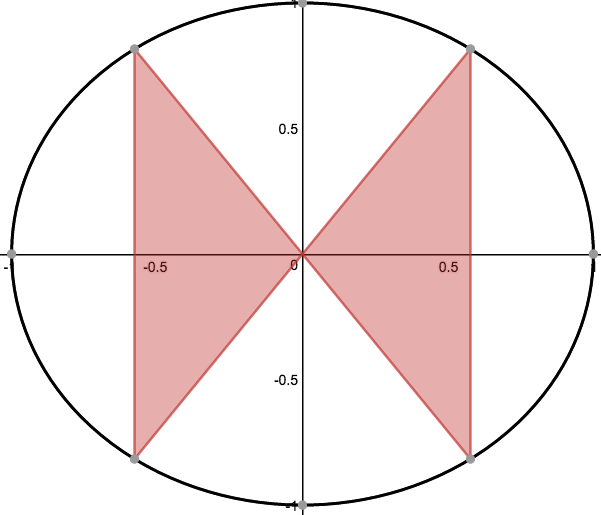
\includegraphics[width=\textwidth]{Circles-3.png}
            \caption{Drawing for Theorem 3.2.15}
          \end{subfigure}
          \begin{subfigure}[b]{0.49\textwidth}
            \centering
            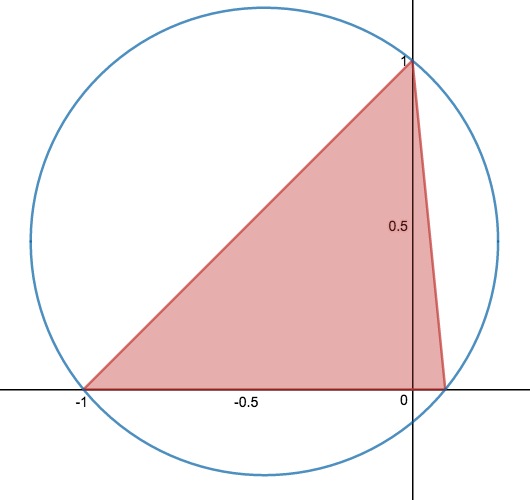
\includegraphics[width=\textwidth]{Circle-4.png}
            \caption{Drawing for Theorem 3.2.16}
          \end{subfigure}
        \end{figure}
        \begin{theorem}
        There exist compact convex sets in $\mathbb{R}^2$ such that $D(K) < 2R_K$.
        \end{theorem}
        \begin{proof}
        For consider the set $K=\{(x,y)\in \mathbb{R}^2: [0\leq y\leq x+1 \land x\geq 0]\lor [0\leq y\leq -10x+1\land x\geq 0]\}$. From Euclid, the smallest circle containing this triangle is the one defined by the three vertices (Three points define a triangle). This circle has the formula $(x+0.45)^2+(y-0.45)^2 = (0.45)^2 +(0.45+\frac{1}{10})^2$. Thus, $2R_K = \sqrt{0.45^2 +(0.45+\frac{1}{10})^2} > \sqrt{2} = D(K)$.
        \end{proof}
        \begin{theorem}
        If $K$ is a compact convex set in $\mathbb{R}^2$, then $D(K) \leq 2R_K$.
        \end{theorem}
        \begin{proof}
        For suppose not. Suppose $D(K) > 2R_K$. As $K$ is compact, there are points $x$ and $y$ in $K$ such that $d(x,y)=D(K)$. But then $d(x,y)>2R_K$, and thus at least one of $x$ or $y$ is not contained in the circle. A contradiction. Thus $D(K)\leq 2R_K$.
        \end{proof}
        \begin{theorem}
        If $K$ is a compact convex set in $\mathbb{R}^2$, then $2\pi r_K \leq P(K)$.
        \end{theorem}
        \begin{proof}
        From Calculus of Variations we know that the circle maximizes the area contained with a set of perimeter $p$. As the inscribed circle has perimeter $2\pi r_K$ and as the circle is a subset of $K$, it is true that $A(K)$ is greater than or equal the area of the circle. Thus, $P(K)\geq 2\pi r_K$.
        \end{proof}
        \begin{theorem}
        For a compact convex set of $\mathbb{R}^2$, $P(K) \leq 2\pi R_K$.
        \end{theorem}
        \begin{proof}
        As $K$ is convex, $P(K) = \pi W(K) \leq \pi \check{W}(K) = \pi D(K) \leq 2\pi R_K$.
        \end{proof}
        \begin{theorem}
        If $K$ is a compact and convex subset of $\mathbb{R}^2$, then $2D(K)\leq P(K)$.
        \end{theorem}
        \begin{proof}
        Suppose not. Suppose $2D(K) >P(K)$. As $K$ is compact and convex, there exist points $x,y\in K$ such that $d(x,y) = D(K)$. But as $K$ is convex, the line contained between $x,y$ in contained in $K$. Thus, $P(\overline{xy}) = 2D(K)$. But as $\overline{xy}\subset K$, $P(K)>P(\overline{xy})$, a contradiction. Thus, $2D(K) \leq P(K)$.
        \end{proof}
        \begin{theorem}
        There exist compact convex subsets of $\mathbb{R}^2$ such that $2D(K) = P(K)$.
        \end{theorem}
        \begin{proof}
        For take a straight line segment of length $\ell$. Then $D(K) = \ell$, $P(K) = 2\ell$, and thus $2D(K) = P(K)$.
        \end{proof}
        \begin{theorem}
        If $K$ is a compact convex subset of $\mathbb{R}^2$, then $P(K) \leq \pi D(K)$.
        \end{theorem}
        \begin{proof}
        From Cauchy's Perimeter theorem, $P(K) = \pi W(K) \leq \pi \check{W}(K) = \pi D(K)$.
        \end{proof}
        \begin{theorem}
        For a compact convex subset $K$ of $\mathbb{R}^2$, $P(K) = \pi D(K)$ if and only if $W_{\ell}(K)$ is a constant.
        \end{theorem}
        \begin{proof}
        For then $\frac{1}{2\pi} \int_{0}^{2\pi} W_{\ell_{\theta}}(K) d\theta = \check{W}(K)$. But as $W_{\ell_{\theta}}(K)$ is continuous for compact convex bodies, it must be true that $W_{\ell_{\theta}}(K) = \check{W}(K)$ for all $\ell_{\theta}$. Thus, $K$ is of constant width.
        \end{proof}
        \begin{remark}
        There are many types of shapes that have constant width besides discs. The Reuleaux Triangle is such an example.
        \end{remark}
        Triangles are the simplest convex bodies in the plane other than points and lines. Any convex polygon can be written as the union of triangles with disjoint interiors. 
        \begin{theorem}
        If $\Delta_s$ is an equilateral triangle with edge length $s$, then $\Delta_s$ has the following properties:
        \begin{enumerate}
        \begin{multicols}{5}
        \item $A(\Delta_s) = \frac{\sqrt{3}}{4}s^2$
        \item $P(\Delta_s) = 3s$
        \item $W(\Delta_s) = \frac{3s}{\pi}$
        \item $R_{\Delta_s} = \frac{1}{\sqrt{3}}s$
        \item $r_{\Delta_s} = \frac{1}{2\sqrt{3}}s$
        \end{multicols}
        \end{enumerate}
        \end{theorem}
        \begin{proof}
        In order:
        \begin{enumerate}
            \item From Pythagoras, $A(\Delta_s) =2\times\big[\frac{1}{2}(\frac{1}{2}s)(\frac{\sqrt{3}}{2}s)\big] = \frac{\sqrt{3}}{4}s^2$
            \item There are three edges, each of length $s$, and thus $P(\Delta_s) = 3s$.
            \item $W(\Delta_s) = \frac{1}{\pi}P(\Delta_s) = \frac{3s}{\pi}$
            \item The circumcircle gives the following equations:
            \begin{enumerate}
                \item $R_{\Delta_s}^2=\frac{s^2}{4}+h^2$
                \item $h+R_{\Delta_s} = \frac{\sqrt{3}}{2}s$
            \end{enumerate}
            This has solution $R_{\Delta_s}=\frac{1}{\sqrt{3}}s$
            \item $r_{\Delta_s} = \frac{R_{\Delta_s}}{2}= \frac{1}{2\sqrt{3}}s$
        \end{enumerate}
        \end{proof}
        \begin{theorem}
        If $T$ is a triangle in the plane, then there is a linear transformation $\psi$ such that $\psi T$ is equilateral.
        \end{theorem}
        \begin{proof}
        For let $T$ be a triangle with vertices $a=(x_1,y_1)$, $b=(x_2,y_2)$, $c=(x_3,y_3)$. Let $A = d(b,c)$, $B=d(a,c)$, and $C=d(a,b)$. Suppose If $A=B=C$, we are done. Thus, suppose $C\geq B >A$. At point $a$ and with radius $C$, construct the circle $b,c',d$, and point $b$ and with radius $C$, construct the circle $a,c',e$. If we can shift $c$ to $c'$ in a linear fashion, we are done. Let $\psi =$
        \end{proof}
        \begin{theorem}
        If $T$ is a triangle with edges $a,b,c$ and opposite angles $\alpha,\beta,\gamma$, respectively, then $A(T) = \frac{\sin(\alpha)}{2}bc = \frac{\sin(\beta)}{2}ac = \frac{\sin(\gamma)}{2}ab$
        \end{theorem}
        \begin{proof}
        Suppose the triangle is acute. The proof is symmetric for all sides, so we prove it for just $\alpha$. Note that the perpendicular $h$ dropped from the vertex of $a$ onto $b$ satisfies $h^2+\ell_1^2 = c^2$ and $h^2+\ell_2^2 = a^2$, where $\ell_1+\ell_2 = b$. Then $\sin(\alpha) = \frac{h}{c}$ and $A(T) = \frac{1}{2}h\ell_1 + \frac{h}{2}h\ell_2 = \frac{h}{2}(\ell_1+\ell_2)h = \frac{1}{2}bh = \frac{1}{2}bc\sin(\alpha)$. An identical argument works for obtuse triangles.
        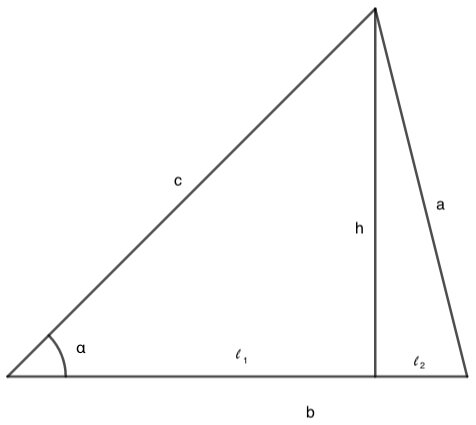
\includegraphics[scale=0.3]{triangle-1.png}
        \end{proof}
        \begin{corollary}[The Law of Sines]
        For a triangle with edges $a,b,c$ and opposite angles $\alpha,\beta,\gamma$, $\frac{\sin(\alpha)}{a} = \frac{\sin(\beta)}{b} = \frac{\sin(\gamma)}{c}$
        \end{corollary}
        \begin{proof}
        From the previous theorem, divide by $\frac{abc}{2}$ to obtain the result.
        \end{proof}
        \begin{theorem}[The Law of Cosines]
        Given a triangle with lengths $a,b,c$ and opposite edges $\alpha,\beta,\gamma$, $c^2=a^2+b^2-2ab\cos(\gamma)$.
        \end{theorem}
        \begin{proof}
        If $\gamma=\frac{\pi}{2}$, this is Pythagoras' Theorem. Thus, suppose $0<\gamma < \frac{\pi}{2}$. Where $c$ and $a$ meet, drop a perpendicular onto $c$ and call this $h$. $h$ satisfies $h^2+\ell_1^2 = c^2$ and $h^2+\ell_2^2=a^2$ from Pythagoras' Theorem, where $\ell_1+\ell_2 = b$. But $\ell_2 = a\cos(\gamma)$, so $\ell_1 = b-a\cos(\gamma)$. Thus $c^2 = h^2 + b^2 +a^2\cos^2(\gamma)-2ab\cos(\gamma)$. But $h = a\sin(\gamma)$. Thus, $c^2 = b^2 + a^2 \cos^2(\gamma)+\sin^2(\gamma)-2ab\cos(\gamma) = b^2 + a^2(\sin^2(\gamma)+\cos^2(\gamma))-2ab\cos(\gamma) = a^2 + b^2 -2ab\cos(\gamma)$. A similar construction is done if $\frac{\pi}{2}<\gamma < \pi$.
        \end{proof}
        \begin{theorem}
        Given a triangle $\Delta$ with lengths $a\leq b\leq c$, $D(\Delta)=c$.
        \end{theorem}
        \begin{proof}
        At the midpoint of $c$, and with radius $c$, construct a circle. This circle contains the entirety of $\Delta$, and thus for all points $x,y\in \Delta$, $d(x,y)\leq c$. Thus, $c=D(\Delta)$.
        \end{proof}
        \begin{theorem}[Heron's Formula]
        For a triangle with lengths $a,b,c>0$, $A(T)^2 = \frac{1}{16}(a+b+c)(-a+b+c)(a-b+c)(a+b-c)$.
        \end{theorem}
        \begin{proof}
        For $A(T) = \frac{1}{2}ab \sin(\gamma) = \frac{1}{2}ab\sqrt{1-\cos^2(\gamma)} = \frac{1}{4}\sqrt{4a^2 b^2 - (a+b-c)^2}=\\ \frac{1}{4}\sqrt{(2ab-(a^2+b^2-c^2))(2ab+(a^2+b^2+c^2))} = \frac{1}{4}\sqrt{(c^2-(a-b)^2)((a+b)^2-c^2)} = \\ \frac{1}{4}\sqrt{(a+b+c)(-a+b+c)(a-b+c)(a+b-c)}$. Squaring this gives the result.
        \end{proof}
        \begin{theorem}
        For any triangle $\Delta$, $r_{\Delta}P(\Delta) = 2A(\Delta)$.
        \end{theorem}
        \begin{proof}
        For let $\Delta$ has sides $a,b,c$, with opposite angles $\alpha, \beta, \gamma$, respectively. Then $A(\Delta) = \frac{ab}{2}\sin(\gamma)$ and $P(\Delta)=a+b+c$. Thus, $\frac{2A(\Delta)}{P(\Delta)} = \frac{ab\sin(\gamma)}{a+b+c}$. But this is the radius of the incircle of $\Delta$. Therefore, etc.
        \end{proof}
        \begin{theorem}[Viviani's Theorem: Page 17]
        \end{theorem}
        \begin{theorem}
        There exist convex polygon's such that the inradius is not unique.
        \end{theorem}
        \begin{proof}
        For consider the rectangle $[0,2]\times [0,1]$. The diameter of any circle that sits inside this body must be at most $1$, and thus the radius is at most $\frac{1}{2}$. However, there are multiple circles that achieve this. For example $(x-\frac{1}{2})^2+(y-\frac{1}{2})^2=\frac{1}{2}$ and $(x-\frac{3}{2})^2+(y-\frac{3}{2})^2=\frac{1}{2}$.
        \end{proof}
        \begin{theorem}
        For an acute triangle, $\frac{2(A)}{abc} = \frac{1}{R_T}$.
        \end{theorem}
        \begin{theorem}
        If $\Delta$ is a triangle with vertices $A,B,C$ and sides $a,b,c$, then given a circle that contains $A,B,C$, the radius of this circle $R$ satisfies $\frac{1}{R} =\frac{2A(\Delta)}{abc}$
        \end{theorem}
        \begin{definition}
        If $K\in \mathscr{K}_2$, then $-K = \{-x:x\in K\}$.
        \end{definition}
        \begin{theorem}
        If $K\in \mathscr{K}_2$, then $W_{\ell}(K) = W_{\ell}(-K)$.
        \end{theorem}
        \begin{proof}
        For let $x,y\in K$ be such that $d(x,y) = W_{\ell}(K)$. Then $d(-x,-y) = W_{\ell}(-K) = d(x,y)$. Therefore, etc.
        \end{proof}
        \begin{theorem}
        There exist sets $K$ and $L$ such that $W_{\ell}(K)<W_{\ell}(L)$ for all $\ell$ yet $K\not\subset L$ for any translation or rotation of $K$.
        \end{theorem}
        \begin{definition}
        For $K\in \mathscr{K}$ and unit vector $u$, $\bar{X}_{u}(K)$ is the mean value of $X_{\ell}(K)$ over all lines $\ell$ parallel to $u$ such that $X_{\ell}(K)>0$.
        \end{definition}
        \begin{theorem}
        For $K\in \mathscr{K}_2$, $\bar{X}_{u}(K) = W_{\ell}(K)=A(K)$.
        \end{theorem}
\end{document}